\documentclass[10pt]{beamer}
% \usepackage[colorlinks=true,citecolor=blue, linkcolor=blue]{hyperref}
\usepackage{hyperref}
\usepackage[utf8x]{inputenc}
% \usepackage{algorithm, algorithmic}
% \usepackage[ruled,vlined]{algorithm2e}
% \usepackage{fontawesome}
\usepackage{graphicx}
% \usepackage[english]{babel}
\usepackage[nodayofweek]{datetime}

\usepackage[colorinlistoftodos]{todonotes}
\usepackage{graphicx}
\usepackage{mathtools}
\usepackage{amssymb}
\usepackage{amsmath}
\usepackage{bbm}
\usepackage{pdflscape}
\usepackage{caption}
\usepackage{subcaption}
\usepackage[T1]{fontenc}
% \usepackage[utf8]{inputenc}
\usepackage{authblk}
\usepackage{pdfpages}
\usepackage{setspace} 
\usepackage{booktabs}
\usepackage{longtable}
\usepackage{float}
\usepackage{tikz}
% \usepackage{multirow}
% \setlength{\tabcolsep}{5pt}
% \usepackage[parfill]{parskip}
% \renewcommand{\arraystretch}{1.5}

% ------------------------------------------------------------------------------
% Use the beautiful metropolis beamer template
% ------------------------------------------------------------------------------
\usepackage[T1]{fontenc}
\usepackage{fontawesome}
\usepackage{FiraSans} 
\mode<presentation>
{
  \usetheme[progressbar=foot,numbering=fraction,background=light]{metropolis} 
  \usecolortheme{default} % or try albatross, beaver, crane, ...
  \usefonttheme{default}  % or try serif, structurebold, ...
  \setbeamertemplate{navigation symbols}{}
  % \setbeamertemplate{caption}[numbered]
  %\setbeamertemplate{frame footer}{My custom footer}
} 

\setbeamertemplate{section in toc}{\hspace*{1em}\inserttocsectionnumber.~\inserttocsection\par}
\setbeamertemplate{subsection in toc}{\hspace*{2em}\inserttocsectionnumber.\inserttocsubsectionnumber.~\inserttocsubsection\par}

% ------------------------------------------------------------------------------
% beamer doesn't have texttt defined, but I usually want it anyway
% ------------------------------------------------------------------------------
\let\textttorig\texttt
\renewcommand<>{\texttt}[1]{%
  \only#2{\textttorig{#1}}%
}

% ------------------------------------------------------------------------------
% minted
% ------------------------------------------------------------------------------
\usepackage{minted}


% ------------------------------------------------------------------------------
% tcolorbox / tcblisting
% ------------------------------------------------------------------------------
\usepackage{xcolor}
\definecolor{codecolor}{HTML}{FFC300}

\usepackage{tcolorbox}
\tcbuselibrary{most,listingsutf8,minted}

\tcbset{tcbox width=auto,left=1mm,top=1mm,bottom=1mm,
right=1mm,boxsep=1mm,middle=1pt}

\newtcblisting{myr}[1]{colback=codecolor!5,colframe=codecolor!80!black,listing only, 
minted options={numbers=left, style=tcblatex,fontsize=\tiny,breaklines,autogobble,linenos,numbersep=3mm},
left=5mm,enhanced,
title=#1, fonttitle=\bfseries,
listing engine=minted,minted language=r}


% ------------------------------------------------------------------------------
% Listings
% ------------------------------------------------------------------------------
\definecolor{mygreen}{HTML}{37980D}
\definecolor{myblue}{HTML}{0D089F}
\definecolor{myred}{HTML}{98290D}

\usepackage{listings}

% the following is optional to configure custom highlighting
\lstdefinelanguage{XML}
{
  morestring=[b]",
  morecomment=[s]{<!--}{-->},
  morestring=[s]{>}{<},
  morekeywords={ref,xmlns,version,type,canonicalRef,metr,real,target}% list your attributes here
}

\lstdefinestyle{myxml}{
language=XML,
showspaces=false,
showtabs=false,
basicstyle=\ttfamily,
columns=fullflexible,
breaklines=true,
showstringspaces=false,
breakatwhitespace=true,
escapeinside={(*@}{@*)},
basicstyle=\color{mygreen}\ttfamily,%\footnotesize,
stringstyle=\color{myred},
commentstyle=\color{myblue}\upshape,
keywordstyle=\color{myblue}\bfseries,
}

% ------------------------------------------------------------------------------
% The Document
% ------------------------------------------------------------------------------

\begin{document}

\title{Developing clustering algorithms for conditional extremes models}

\date{
  \footnotesize Thesis formulation report (TFR) presentation \\ 
  \today \\
  % \shortdate \\
  % \vspace{0.4cm}
  \emph{Paddy O'Toole} \\
  % \vspace{-5mm}
  \emph{Supervised by Christian Rohrbeck and Jordan Richards (University of Edinburgh)}
}

% \title{Wessex Water: Bayesian Network for Source Apportionment}
% \author{\emph{Sam Williams, Paddy O'Toole, Christian Rohrbeck, Haiyan Zheng, Emiko Dupont}}
% \date{\today}


\frame{\titlepage}

%==================================================

% \frame{\begin{small}
% \frametitle{Overview}
% \tableofcontents\end{small}}

%=================================================
\begin{frame}
\frametitle{Table of Contents}
\tableofcontents
\end{frame}

\section{Introduction}

% TODO: Perhaps add one more introduction slide?

% Motivation behind EVT
\begin{frame}{Introduction}
% \todo{Include use cases}
    % \begin{itemize}
    %     \item Extreme Value Theory is a field of statistics concerned with modelling the extremal tail of distributions, where standard methods do not perform well
    %     \item Many use cases, particularly popular for environmental data (rainfall, flooding, storms, temperature), where tail events often catastrophic. 
    %     \item Concerned with performing \textbf{extremal clustering}, helps with dimensionality reduction and understanding patterns in data
    %     % Need to have metric for magnitude over which to deem events as extreme, and then frequency or concommitant extremes for clustering 
    % \end{itemize}

   \begin{minipage}{0.49\textwidth}
        % Anything else to add here?
        \begin{itemize}
            \item Extreme Value Theory models the extreme tails of distributions $X$ % standard models don't work well
            \item Only known method that can reliably predict beyond observations in extremal context
            \item Application fields include finance and insurance, and environmental data, such as extreme precipitation and/or wind speeds. % todo: Rewrite this!
        \end{itemize}
   \end{minipage}
   \hfill
   \begin{minipage}{0.49\textwidth}
     % \centering
     \vspace{}
     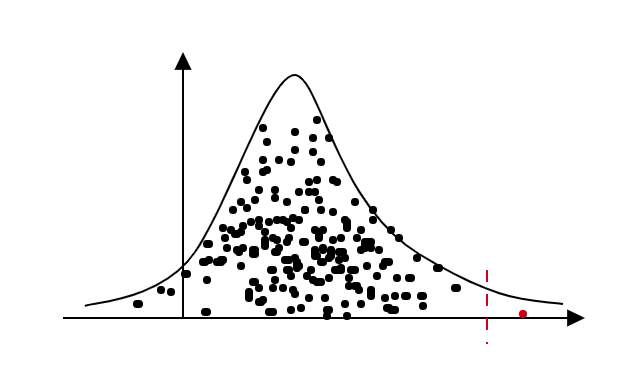
\includegraphics[width=6cm]{images/tail.png}
   \end{minipage}
\end{frame}

% Images of Pulteney Bridge Weir and plaque
% Frank Greenhalgh, Engineer who designed Pulteney Weir and Sluce for Bristol Avon River Authority
\begin{frame}
   \begin{minipage}{0.49\textwidth}
     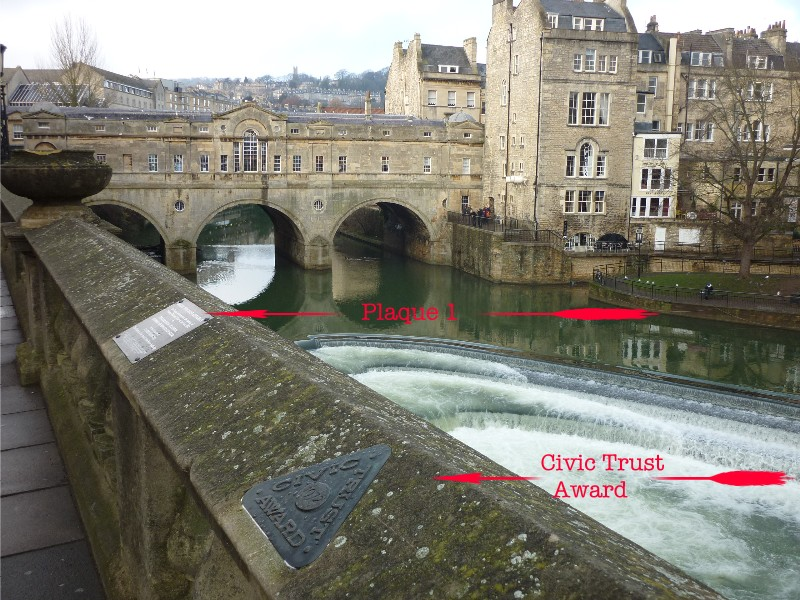
\includegraphics[width=.99\textwidth]{images/civictrustaward_location.jpg}
   \end{minipage}
   \hfill
   \begin{minipage}{0.49\textwidth}
   % todo: Rotate image (and add in!)
     \vspace{}
     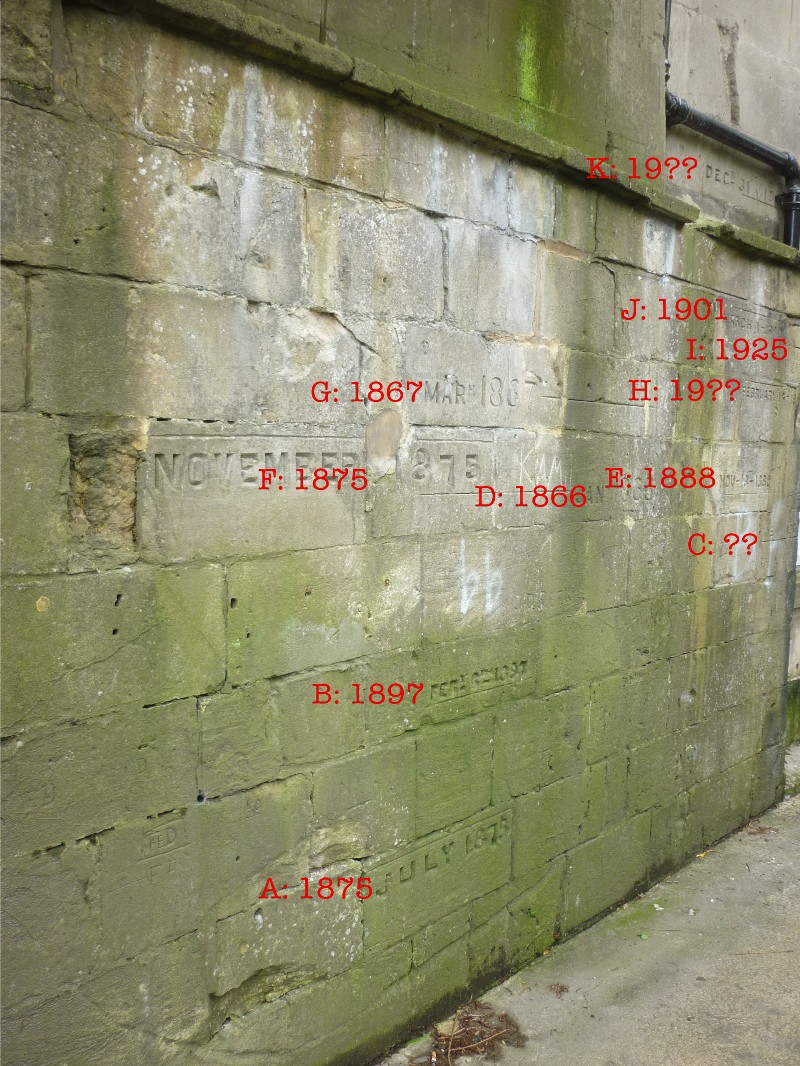
\includegraphics[width=.99\textwidth]{images/Hapennybr_lower.jpg}
   \end{minipage}
\end{frame}

% MV extremes, uses, methods, shortcomings - clustering
% todo: Add 2D plot showing different regions of extremity
\begin{frame}{Multivariate extremes}
    \begin{itemize}
      \item Concurrently occurring extremal events can be particularly destructive 
      \item $\mathbb{P}(\bm{X} \in \bm{C}) = \sum_{i=1}^{d}{\mathbb{P}(\bm{X}_i \in C_i)}$, for some extreme set $C_i$ corresponding to each vector $X_i$. 
      \item This may refer to different spatial locations, or different variables
      \item For example, offshore platforms must be built to withstand extreme wind speed and wave height conditions at sea
      \item Storm defences must withstand extreme rainfall and wind speed conditions, and insurance premiums must take into account these particularly destructive events
    \end{itemize}
\end{frame}

\begin{frame}{Multivariate extremes}
     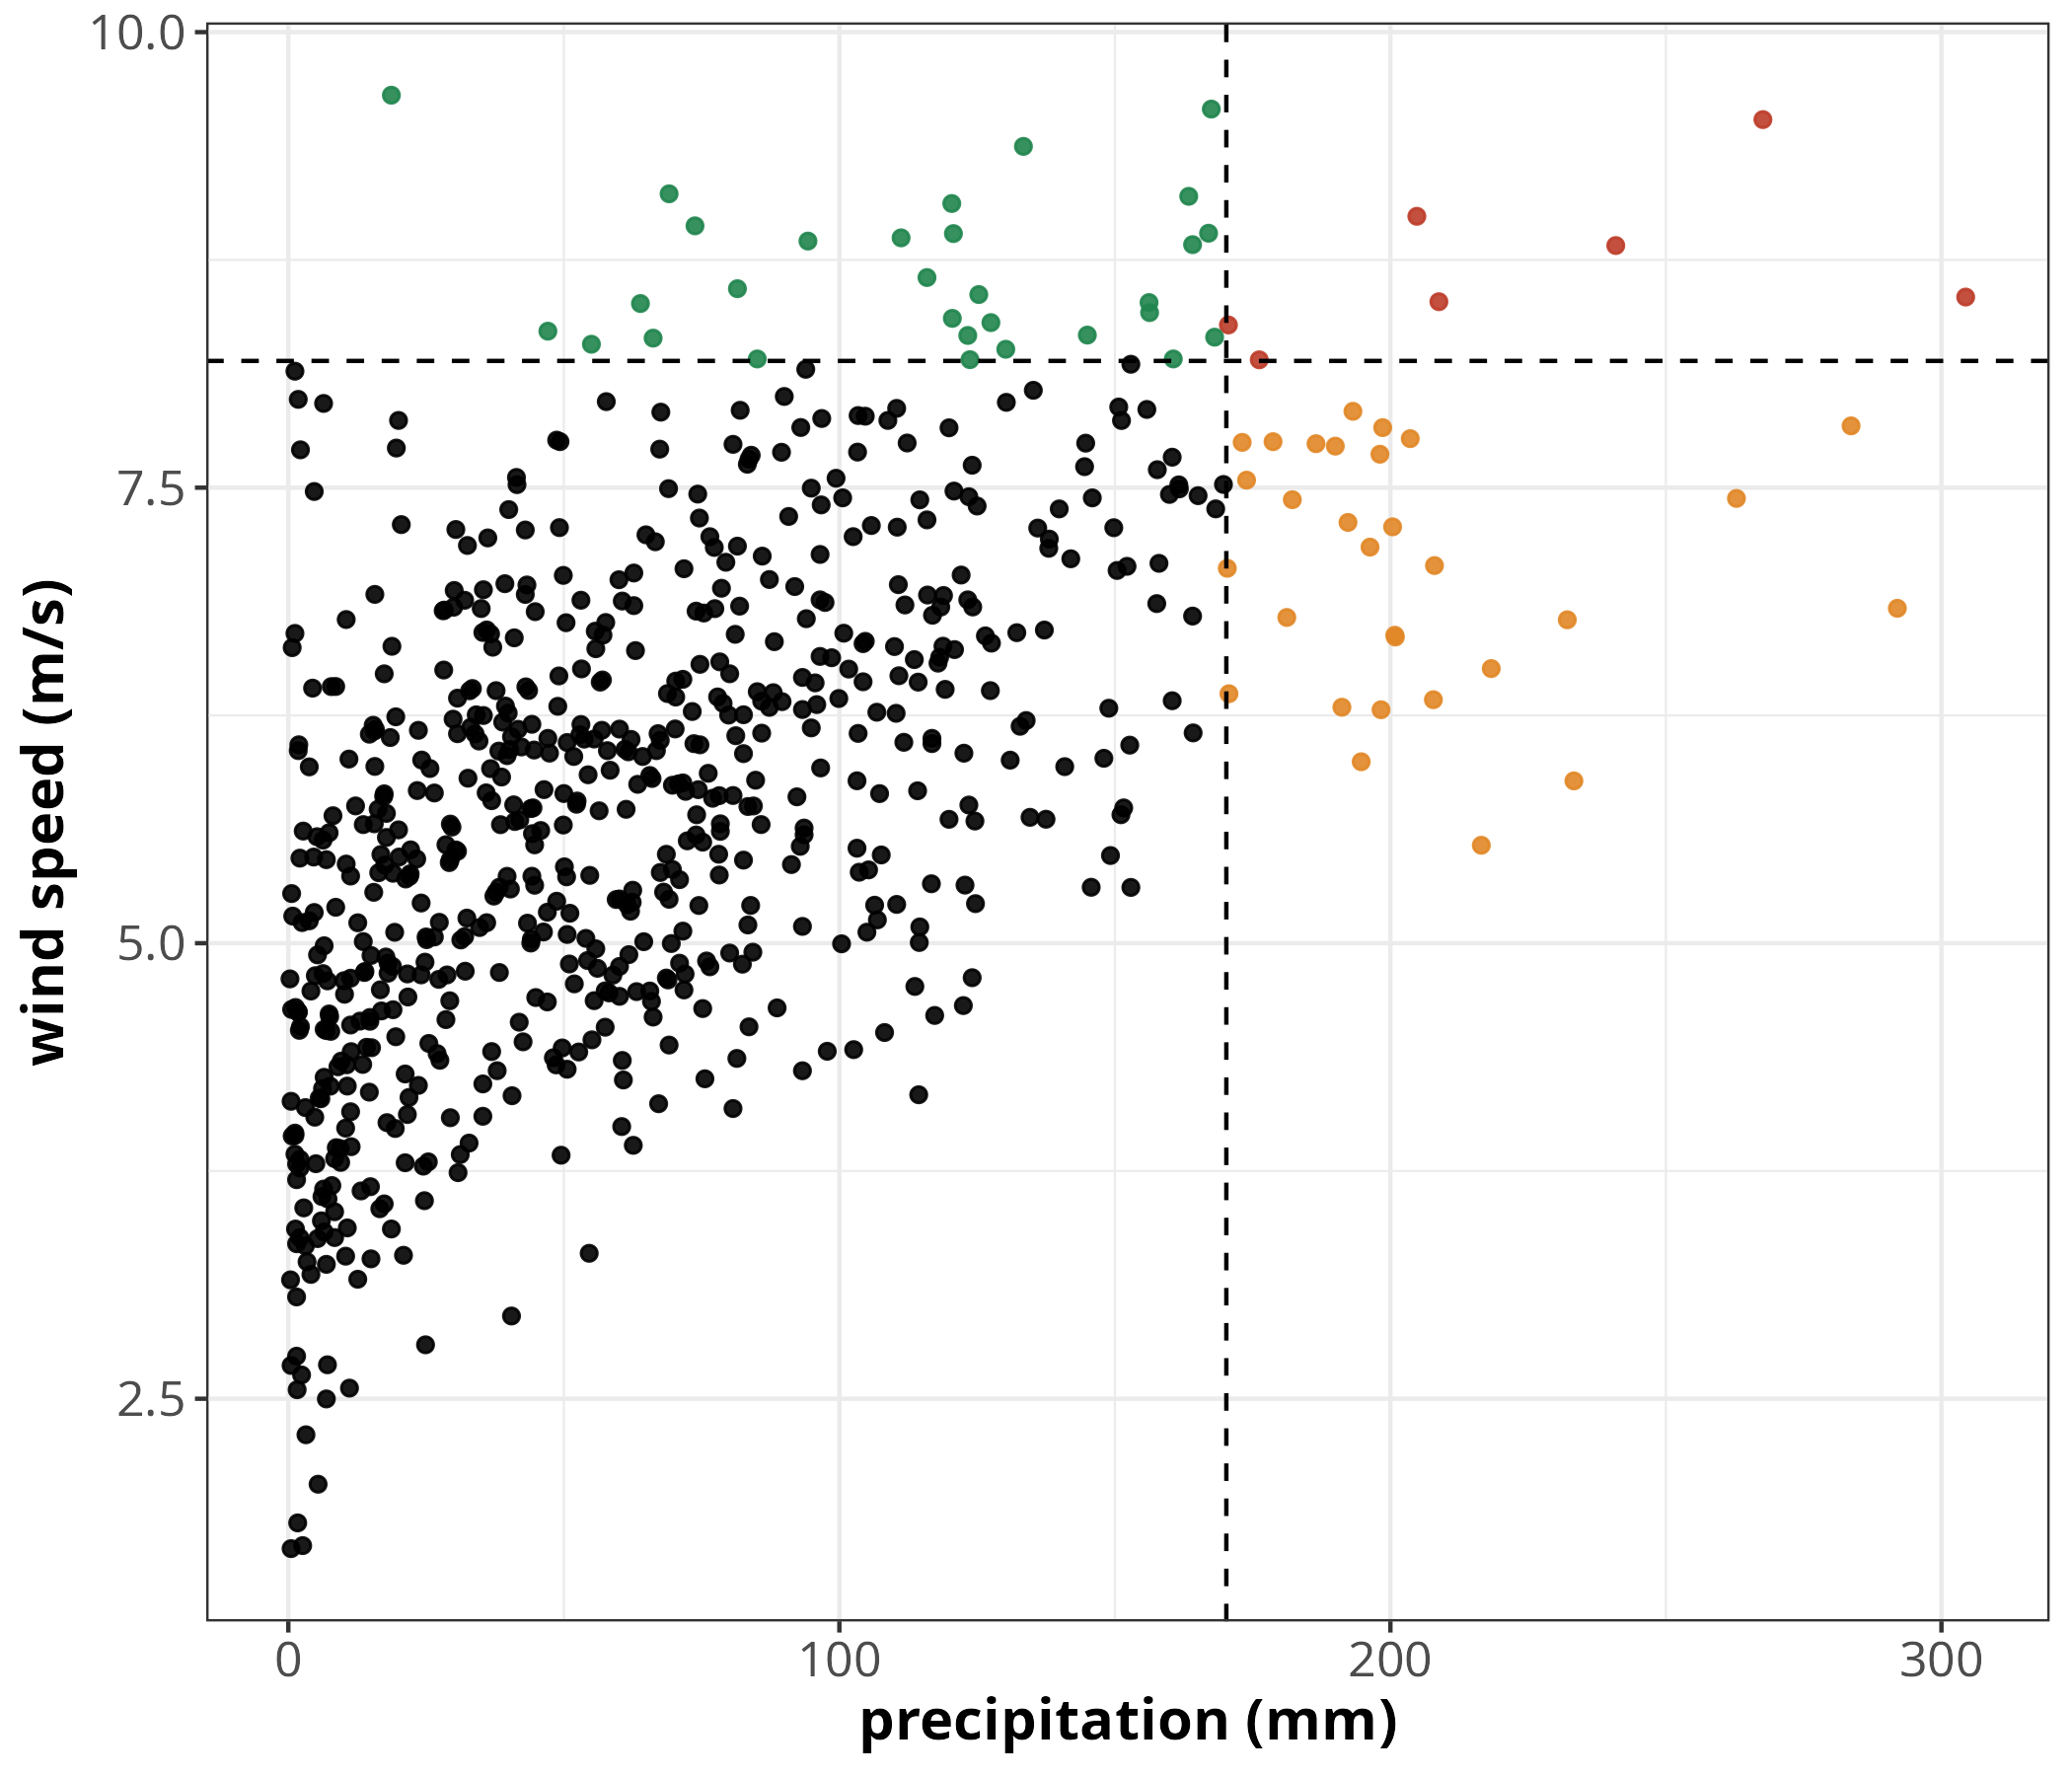
\includegraphics[width=.9\textwidth]{plots/021_mv_extreme.png}
\end{frame}

\section{Motivating example}

% Describe motivating example
\begin{frame}{Motivating example - Ireland}

   \begin{minipage}{0.49\textwidth}
       \begin{itemize}
           \item Extreme precipitation and wind speed in Ireland, 1990-2020
           \item Precipitation data from 52 Met Éireann weather sites across country, wind data from ERA5 reanalysis dataset.
           \item Take weekly sum of precipitation and mean of daily wind speed maxima for Winter only (Oct-Mar), in line with Vignotto et.\ al.\ (2021) \cite{Vignotto2021}. % todo: Fix citations
       \end{itemize}
   \end{minipage}
   \begin{minipage}{0.49\textwidth}
     \vspace{}
     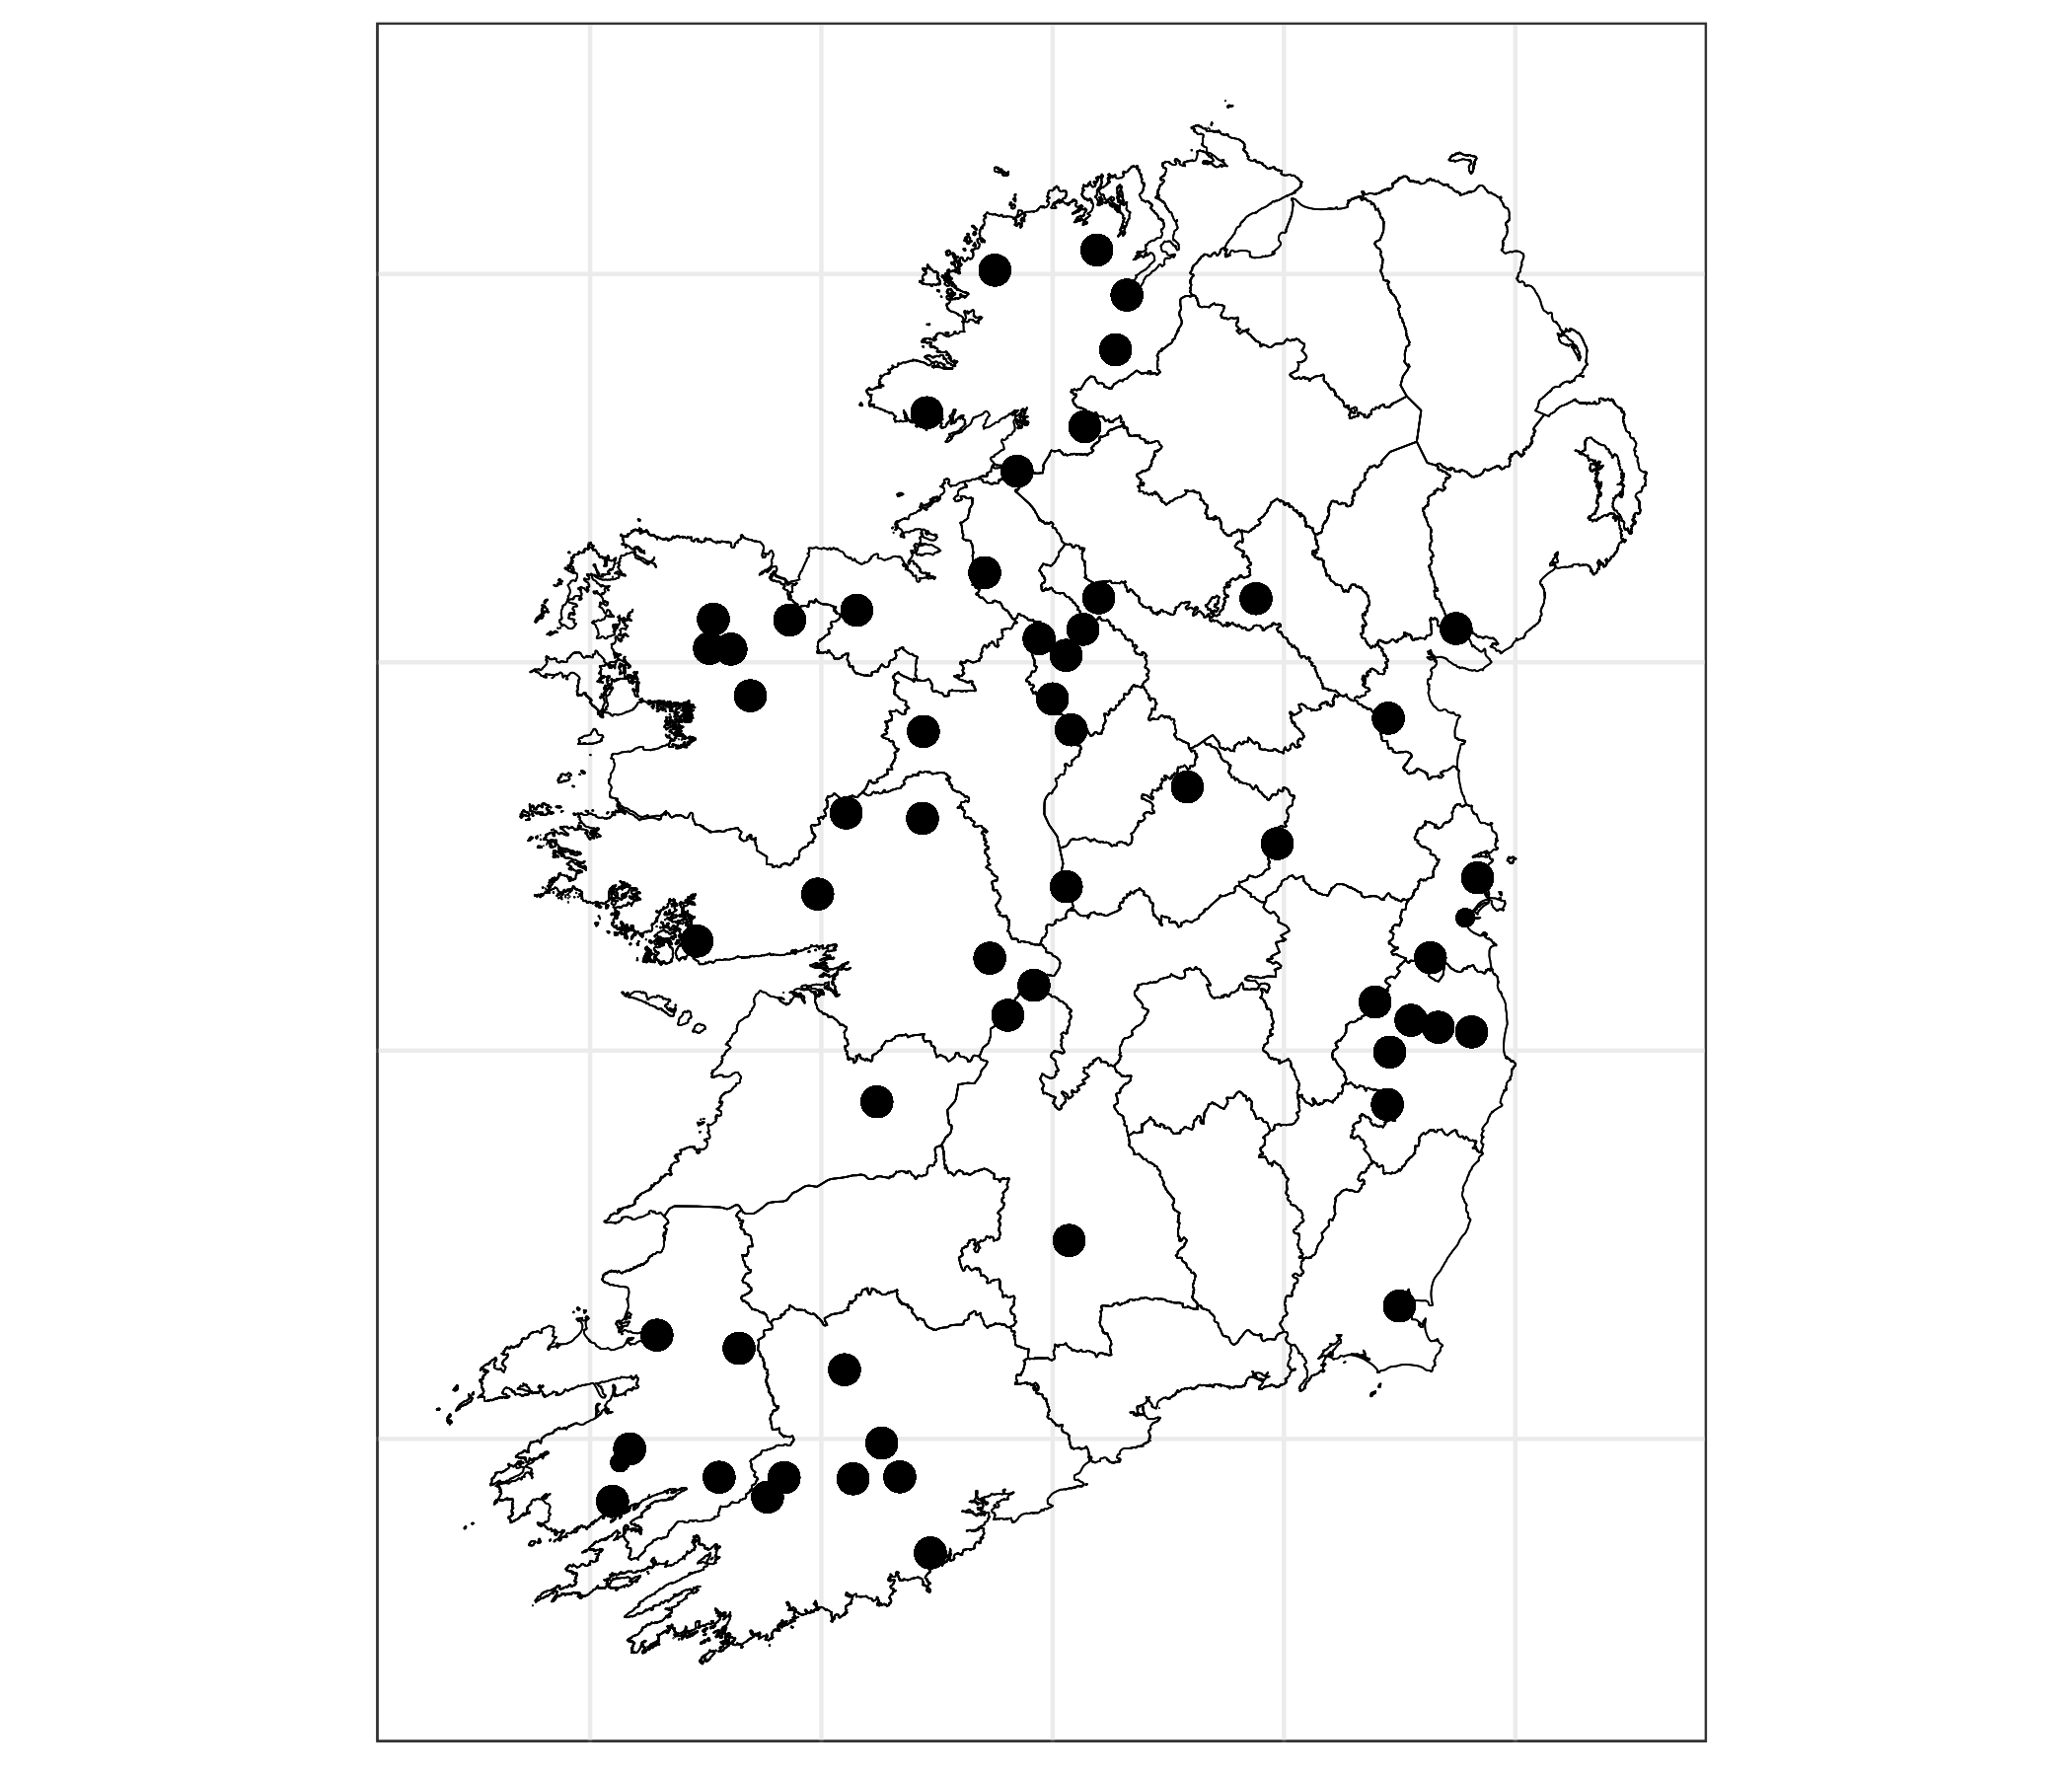
\includegraphics[width=7cm]{plots/01_ire_plot.png}
   \end{minipage}
\end{frame}

\section{Univariate extremes}


% GPD formula, threshold selection, non-stationary version
\begin{frame}{Generalised Pareto distribution}
The Generalised Pareto distribution (GPD) has survival function:
\begin{equation*} 
  % \mathbb{P}(Z \le z + u \mid Z > u) = 1 - \left(1 + \xi \frac{z}{\sigma} \right)_{+}^{-1/\xi},
  \mathbb{P}(X > x + u \mid X > u) = \left(1 + \xi \frac{x}{\sigma} \right)_{+}^{-1/\xi},
\end{equation*}
\vspace{-5mm}
\begin{itemize}
    \item $(x)_+ = \max{(0, x)}$
    \item Scale $\sigma$, shape $\xi$, threshold $u$
    \item For $\xi < 0$, (increasingly small) finite upper end point
    \item Can model parameters as function of spatial location, i.e.\ $\sigma(s), \xi(s)$, with $s =$ (longitude, latitude)
    \item Threshold often taken as high quantile of data, can also model as $u(s)$
\end{itemize}

\end{frame}

% Plot of sigma, xi values across Ireland
\begin{frame}{Motivating example - Precipitation}

% todo: Add horizontal space here
% \hspace{}
% \begin{minipage}{0.49\textwidth}
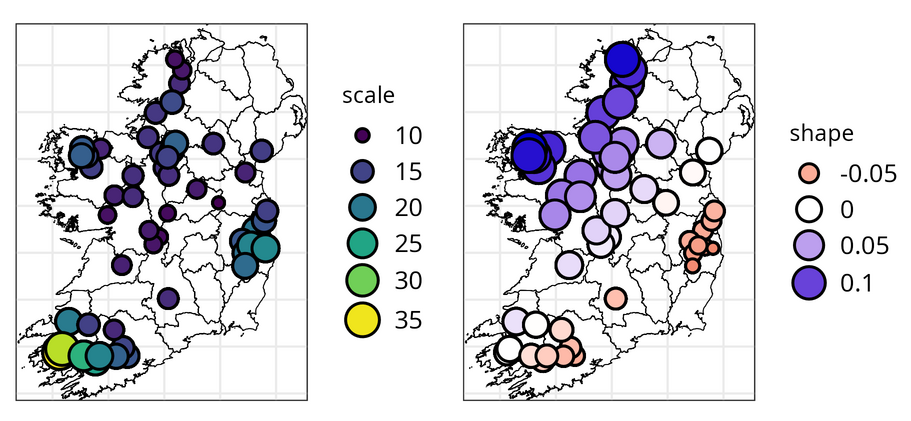
\includegraphics[width=1\textwidth]{plots/032_gpd_rain_crop.png} 
% \end{minipage}
% \vfill
% \begin{minipage}{0.49\textwidth}
%     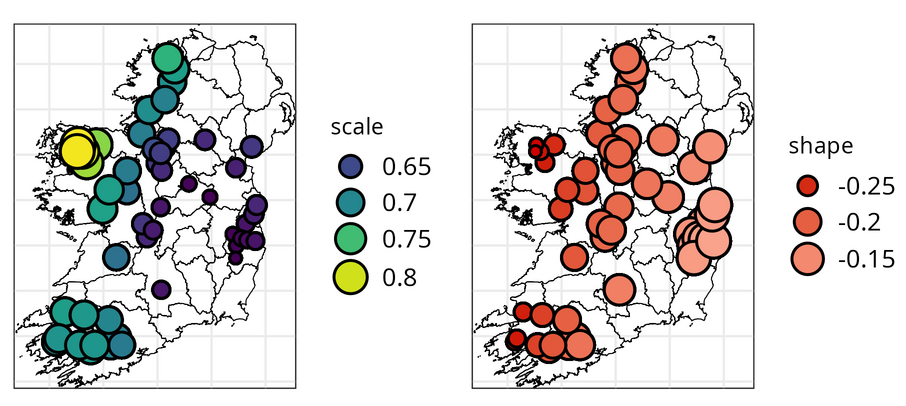
\includegraphics{plots/033_gpd_ws_crop.png} 
% \end{minipage}
\end{frame}

\begin{frame}{Motivating example - Wind speed}
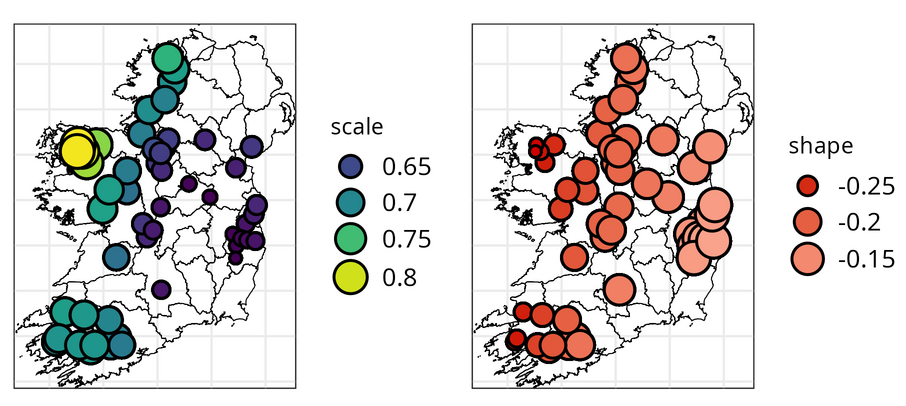
\includegraphics[width=1\textwidth]{plots/033_gpd_ws_crop.png} 
\end{frame}

\begin{frame}{Motivating example - Wind speed}
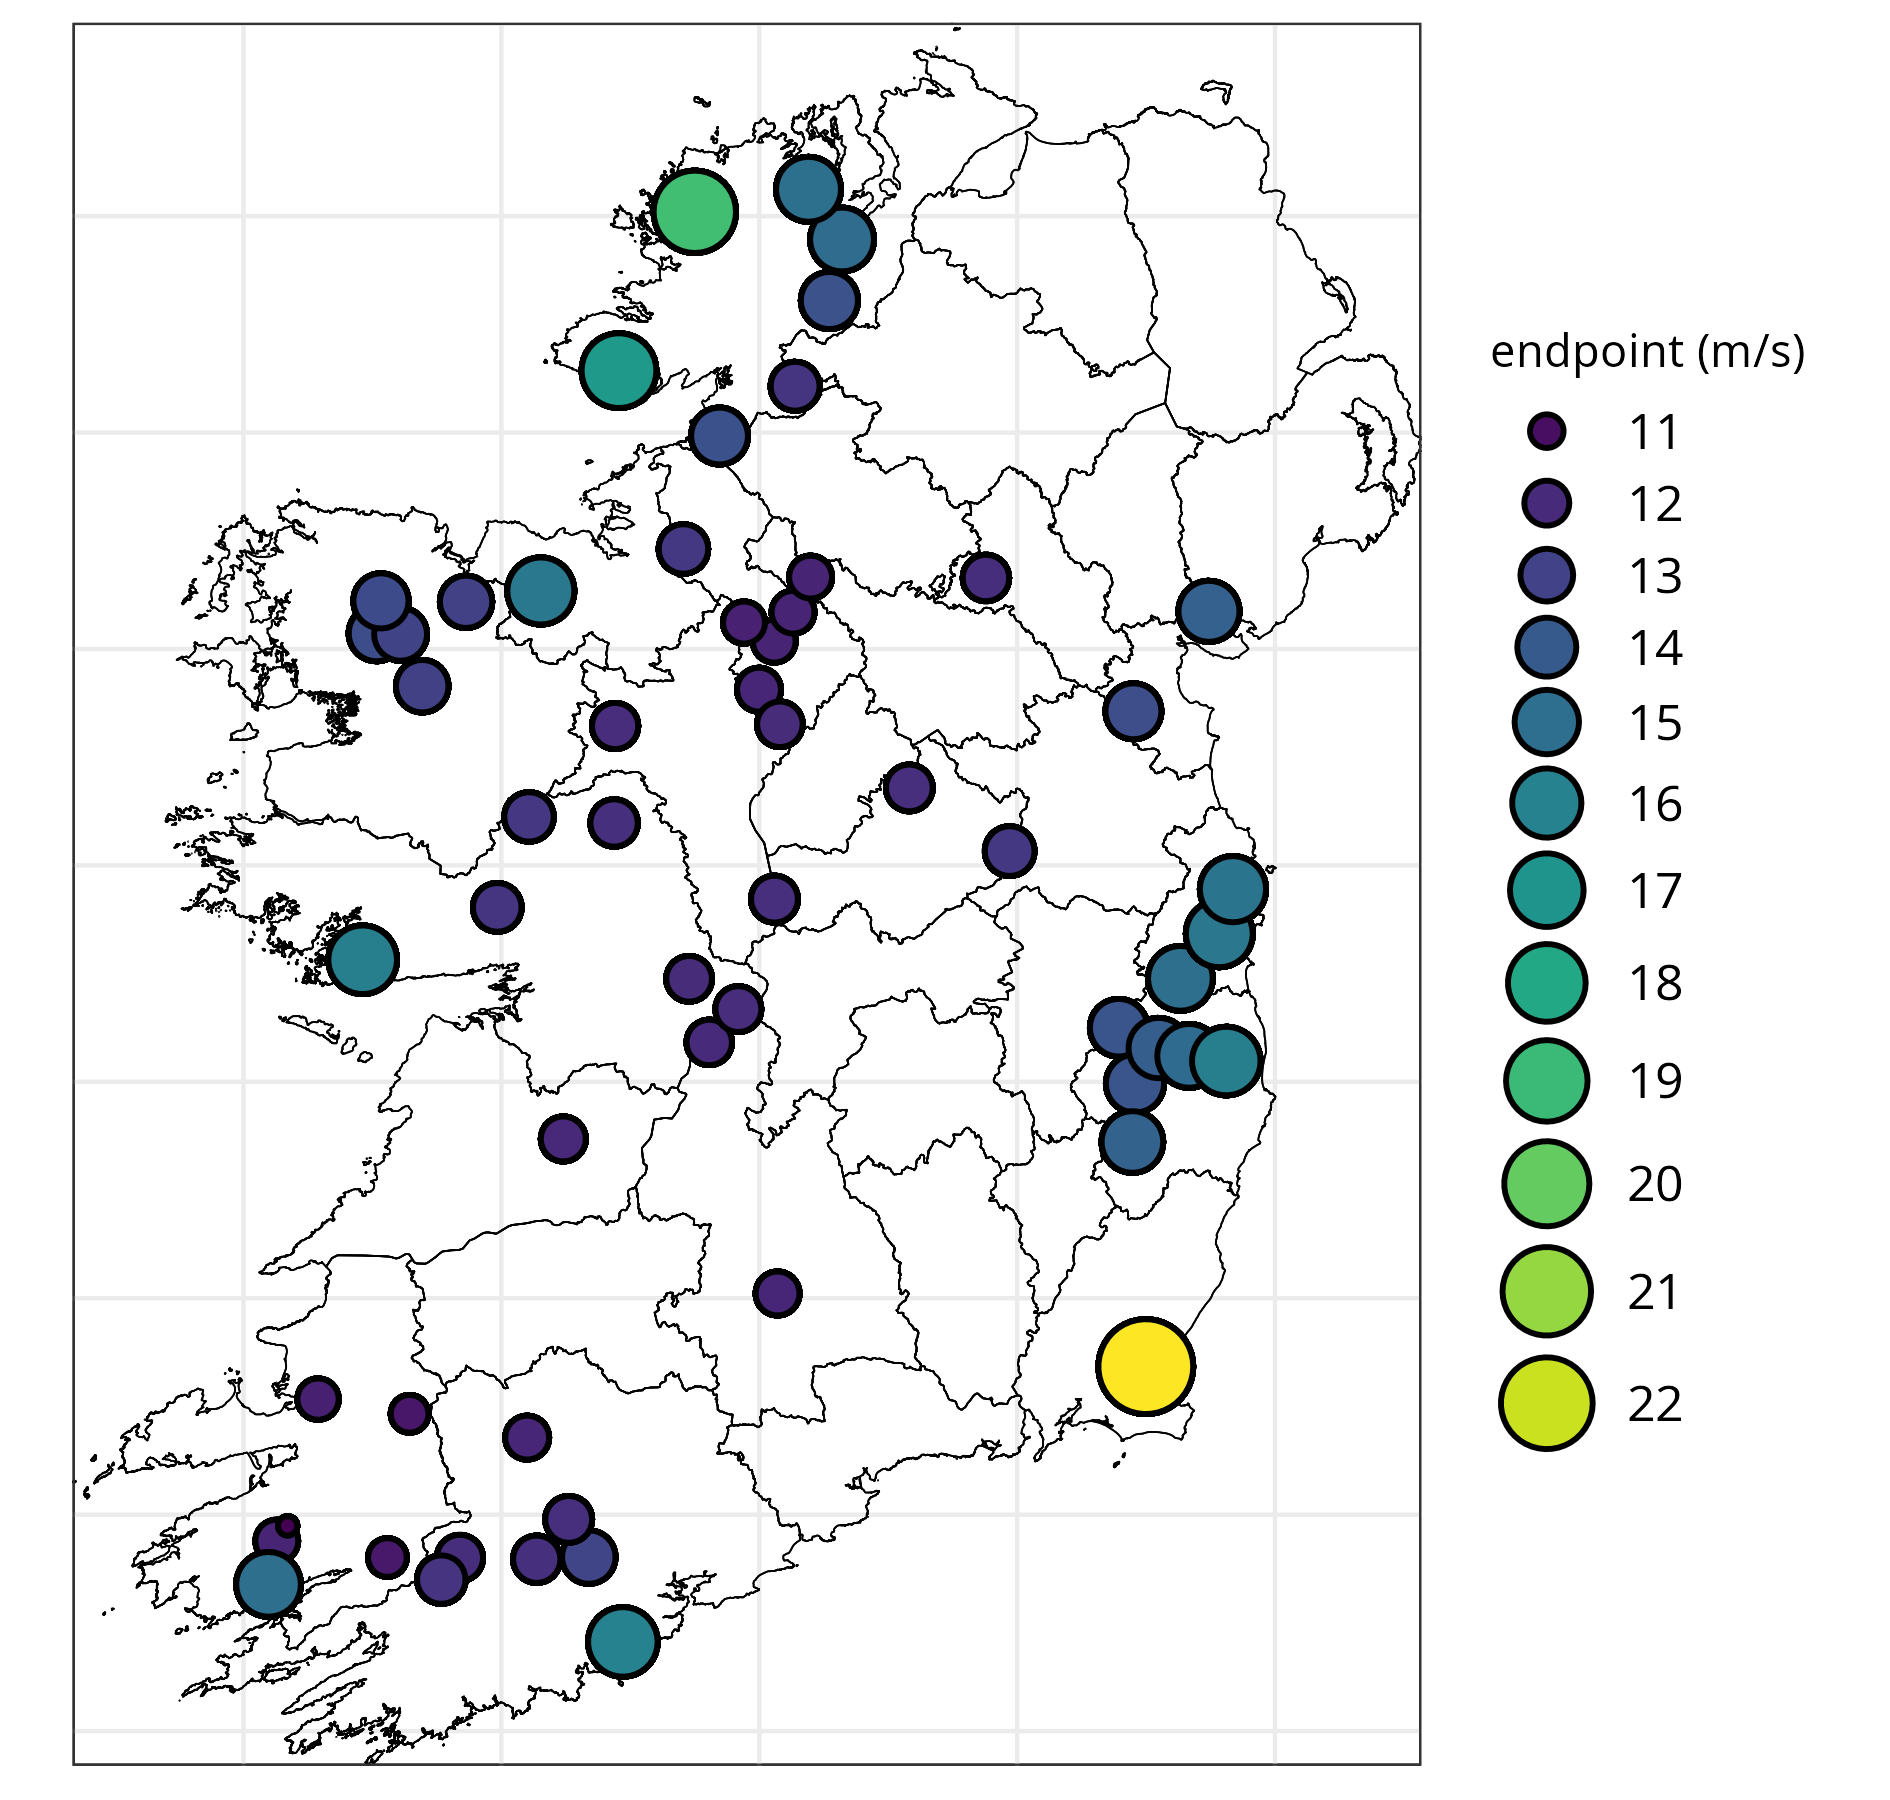
\includegraphics[width=0.8\textwidth]{plots/034_ws_endpoint.png}
\end{frame}

\section{Conditional extremes}
\begin{frame}{Introduction}
% TODO: Define Y_{-i}, Y_{j \mid i}, Y_{\mid i}
\begin{itemize}
    \item Gets name from modelling \emph{conditional} on single variable, e.g.\ precipitation conditional on observing extreme wind speed
    \item Has simple marginal and dependence components
    \item Can model all varieties of extremal dependence, from asymptotic independence (Probability of $X_i$ being extreme is not effected by $X_j$ being extreme) to perfect dependence ($X_i$ is extreme only where $X_j$ is extreme)
    \item Some definitions:
    \begin{itemize}
        \item $\bm{X}_{-i}$: Vector $\bm{X}$ without $i^{th}$ component
        \item $\bm{\alpha}_{\mid i}$: Vector of parameters $\alpha_{j \mid i}$ conditional on $X_i$, $j \ne i$
    \end{itemize}
\end{itemize}
\end{frame}

% Univariate piecewise function
\begin{frame}{Univariate}
Univariate component of model: semi-parametric piecewise function of empirical distribution below threshold and GPD (from previous section) above threshold:
\begin{equation*} 
  \hat{F}_{X_i}(x) = \begin{cases}
    1 - \{ 1 - \tilde{F}_{X_i}(u_{X_i})\} \left\{1 + \xi_{i}(x - u_{X_i})/\sigma_i\right\}_{+}^{-1/\xi_{i}} & \text{if } x > u_{X_i} \\
    \tilde{F}_{X_i}(x) & \text{if } x \le u_{X_i},
  \end{cases}
\end{equation*}
where $\tilde{F}_{X_i}$ is the empirical distribution function of $X_i$.
\end{frame}

% Transform to Laplace
\begin{frame}{Marginal transformation}
Marginals transformed to Laplace margins using probability integral transform:
\begin{equation*}
  Y_i = \begin{cases}
    % \exp(y)/2 &\text{ for } y < 0 \\
    \log\left\{2F_{X_i}(X_i)\right\} &\text{ for } X_i < F_{X_i}^{-1}(0.5), \\
    -\log\left\{2(1 - F_{X_i}(X_i))\right\} &\text{ for } X_i \ge F_{X_i}^{-1}(0.5), \\
  \end{cases}
\end{equation*}
\vspace{-5mm}
\begin{itemize}
    \item transformation denoted $Y_i$ to differentiate from original marginals $\bm{X}$ 
    \item Both tails exponential with mean 1
\end{itemize}
\end{frame}

% Multivariate piecewise function, Z, Y independent
\begin{frame}{Multivariate}
Dependence component of model:
\begin{equation*} 
    % TODO: Define Y_{-i} above
    \bm{Y}_{-i} = \bm{\alpha}_{\mid i}\bm{y}_i + \bm{y}_i^{\bm{\beta}_{\mid i}}\bm{Z}_{\mid i}, \text{ for } Y_i = y_i > u_{Y_i}.
\end{equation*}
\vspace{-5mm}
\begin{itemize}
    \item $\alpha_{j \mid i} \in [-1, 1]$ is slope parameter for $Y_j$ conditional on $Y_i$, $\beta_{j \mid i} \in (-\infty, 1]$ is spread parameter
    \item Residuals $\bm{Z}_{\mid i}$ said to have distribution $\bm{G}_{\mid i}$
    \item $\bm{\beta}_{\mid i}$ controls level of stochasticity of relationship between $\bm{Y}_{-i}$ and large $Y_i$. 
    \item Special cases:
    \begin{itemize}
        \item $\bm{\alpha}_{\mid i} = 0, \bm{\beta}_{\mid i} = 0 \implies \bm{Y}_{-i}, \bm{Y}_{i}$ independent
        \item $\bm{\alpha}_{\mid i} = -1/1, \bm{\beta}_{\mid i} = 0 \implies$ perfect positive/negative dependence
        \item $-1 < \bm{\alpha}_{\mid i} < 1 \implies$ asymptotic independence %todo define above
    \end{itemize}
\end{itemize}
\end{frame}

% Methods for estimation, assumption on Z
\begin{frame}{Estimation}
Common estimation procedure:
    \begin{enumerate} 
        \item First assume $\bm{Z}_{\mid i} \sim N(\mu_{\mid i}, \sigma_{\mid i})$, generate residuals from this distribution
        \item Use likelihood methods to estimate $\hat{\bm{\alpha}}_{\mid i}, \hat{\bm{\beta}}_{\mid i}$, and nuisance parameters $\hat{\mu}_{\mid i}, \hat{\sigma}_{\mid i}$
        \item Estimate $\hat{G}_{\mid i}$ as the empirical distribution of 
       \[
         \bm{Z}_{\mid i} = \frac{\bm{Y}_{-i} - \hat{\bm{\alpha}}_{\mid i}Y_i}{Y_i^{\hat{\bm{\beta}}_{\mid i}}}.
       \]
    \end{enumerate}
    This procedure is very simple, and can easily be used to generate MC samples to calculate desired probabilities
\end{frame}

% Poor results initially, high uncertainty
\begin{frame}{Motivating example - Uncertainty}
\begin{minipage}{0.49\textwidth}
        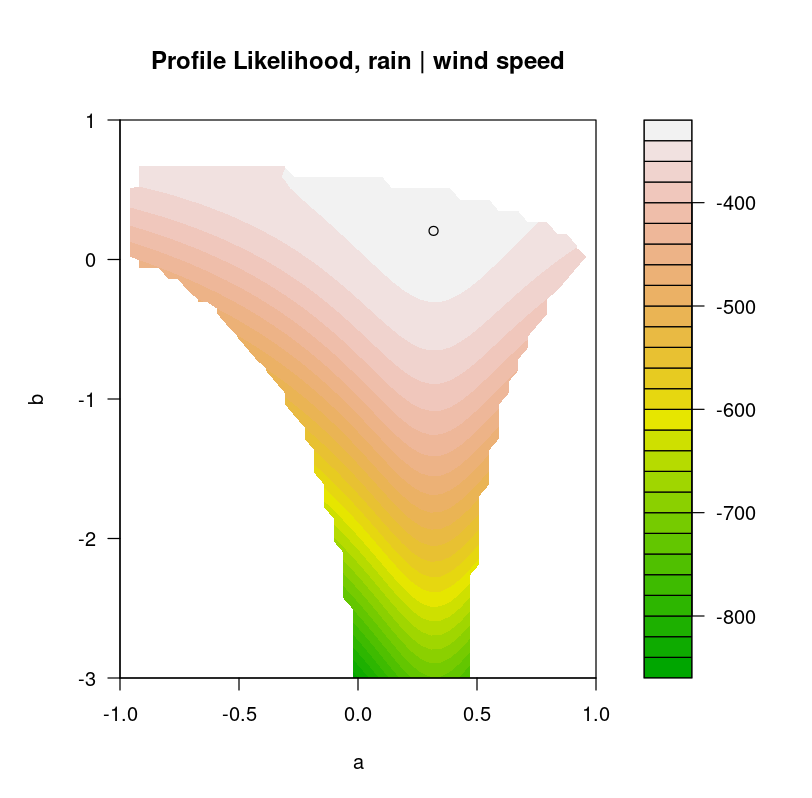
\includegraphics[width=0.99\textwidth]{plots/043_prof_ll.png}
   \end{minipage}
   \hfill
\begin{minipage}{0.49\textwidth}
    \vspace{}
    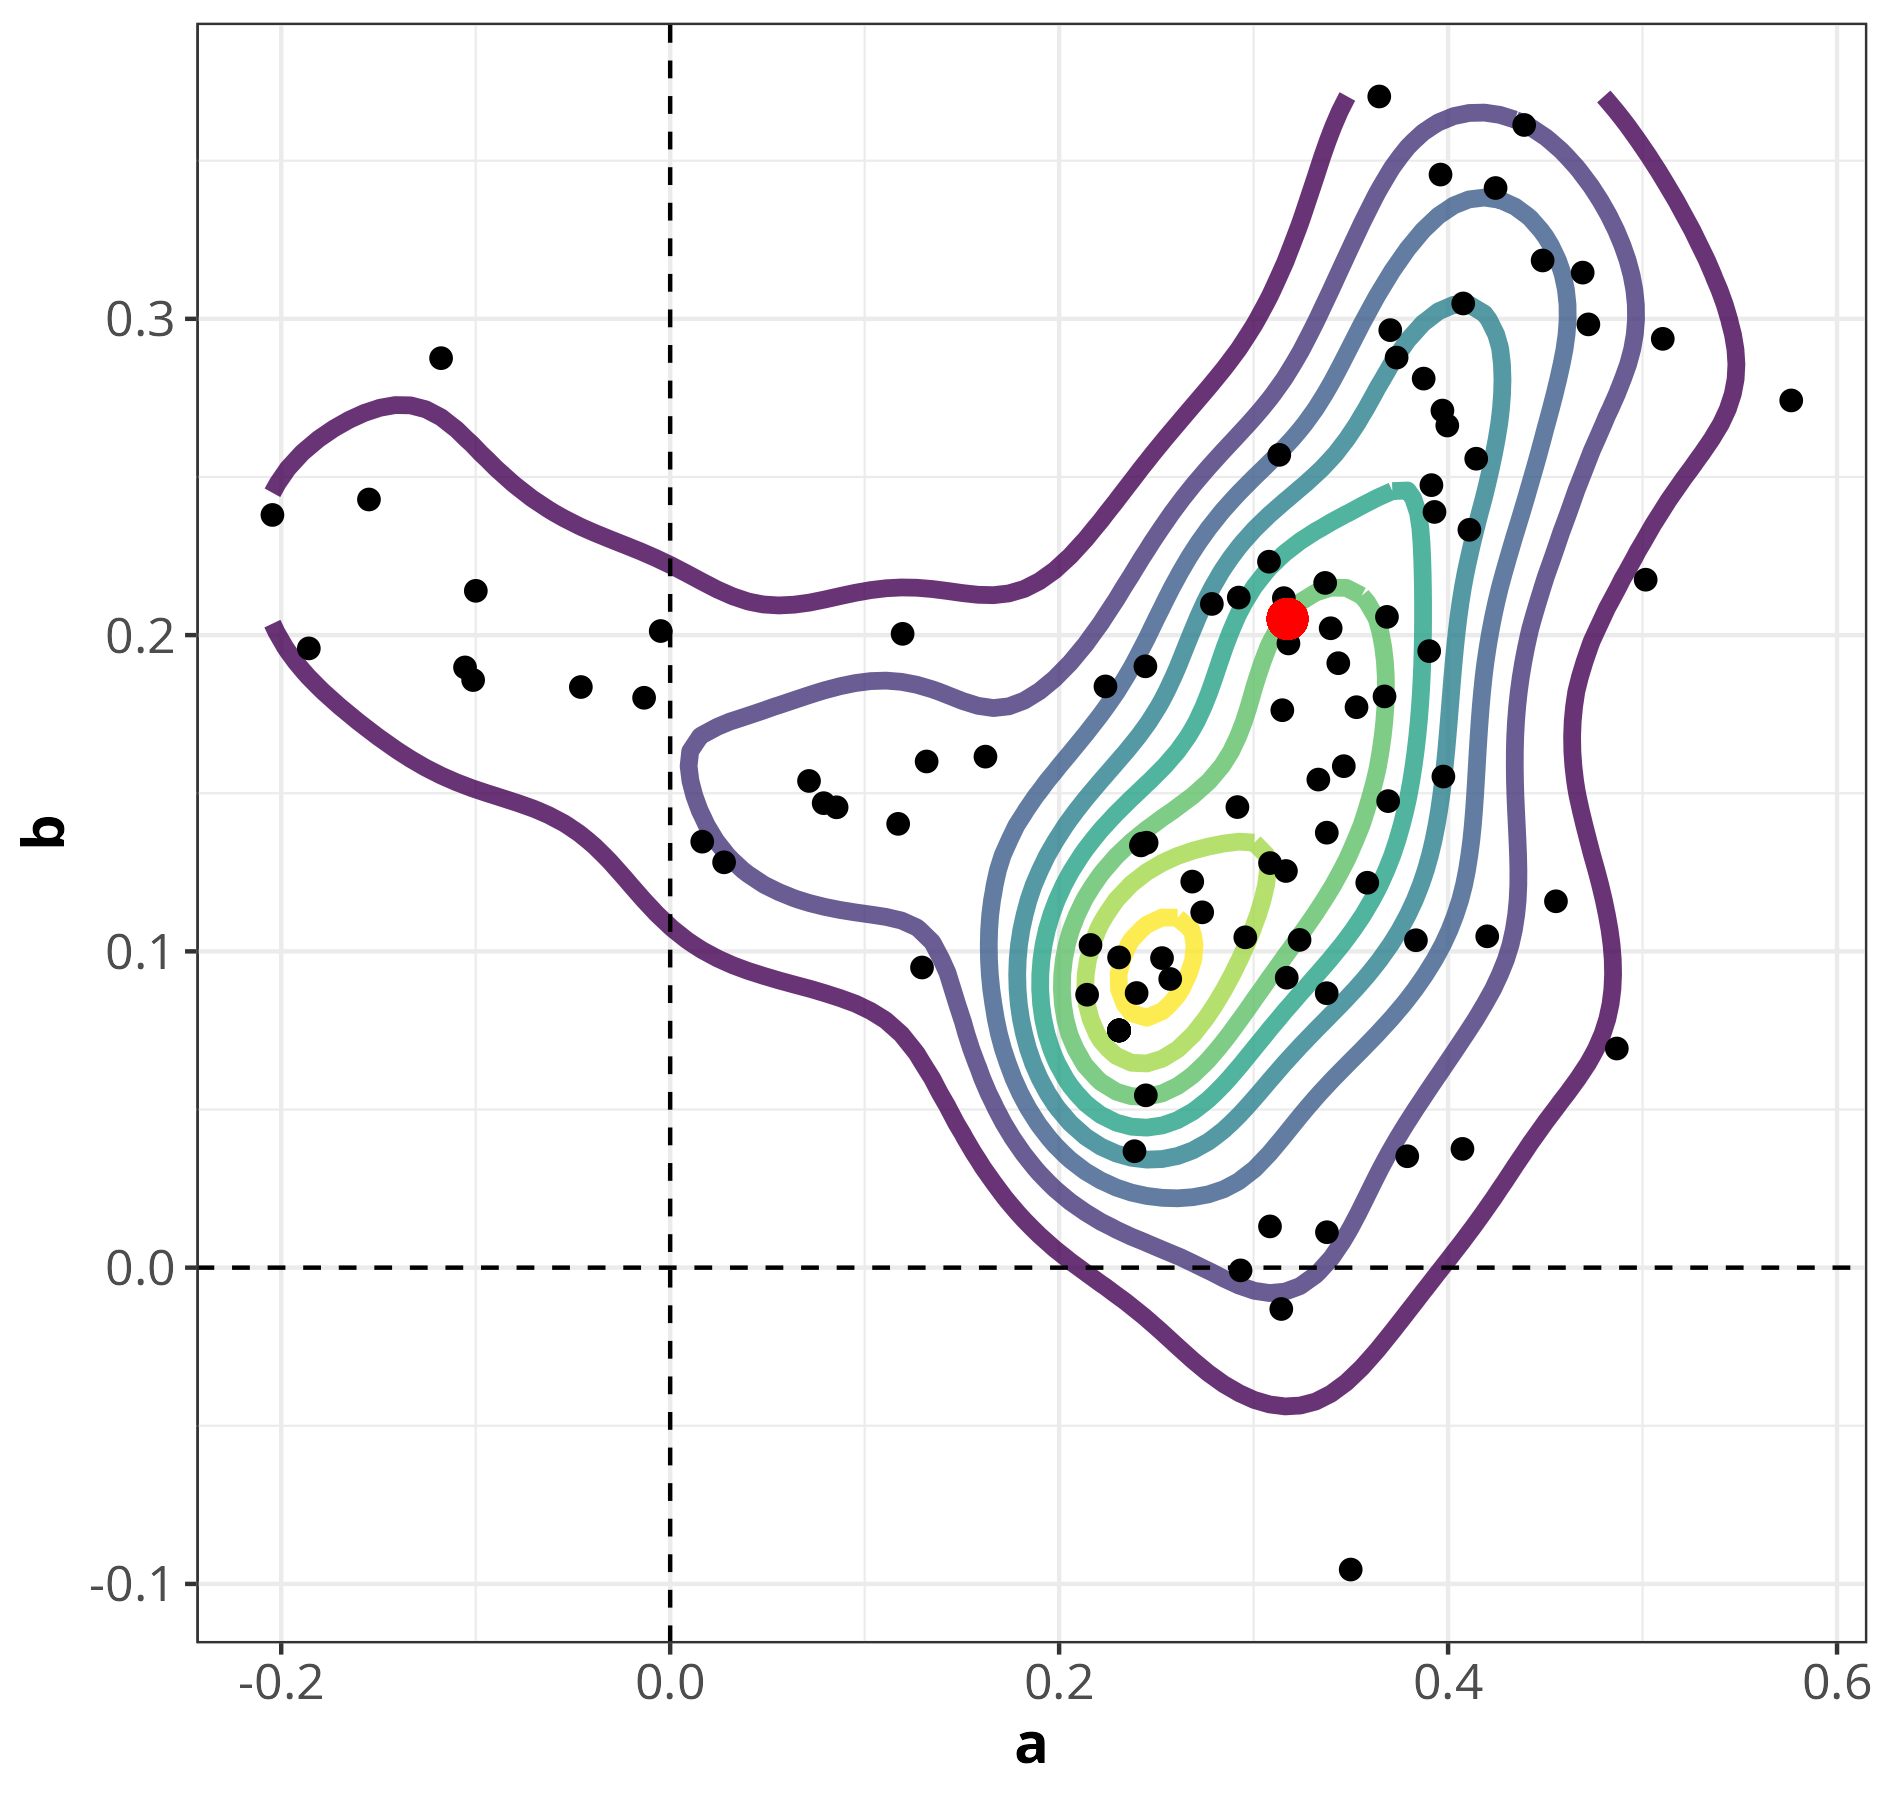
\includegraphics[width=0.99\textwidth]{plots/044_bootstrap_density.png}
\end{minipage}
\end{frame}

% Improved here
\begin{frame}{Fixing $\beta$}
    \begin{itemize}
        \item Problem: Difficult to interpret results while varying both $\alpha, \beta$ due to uncertainty (and negative, unlikely estimates for $\beta$)
        \item ``Hack'': Fix $\beta = 0.1$ (allowing some stochasticity), estimate only $\alpha$
        \item Idea: By estimating only one parameter, should contain all information about extremal dependence, and be more easily interpretable
    \end{itemize}
\end{frame}

% Map of alpha values
\begin{frame}{Results}
    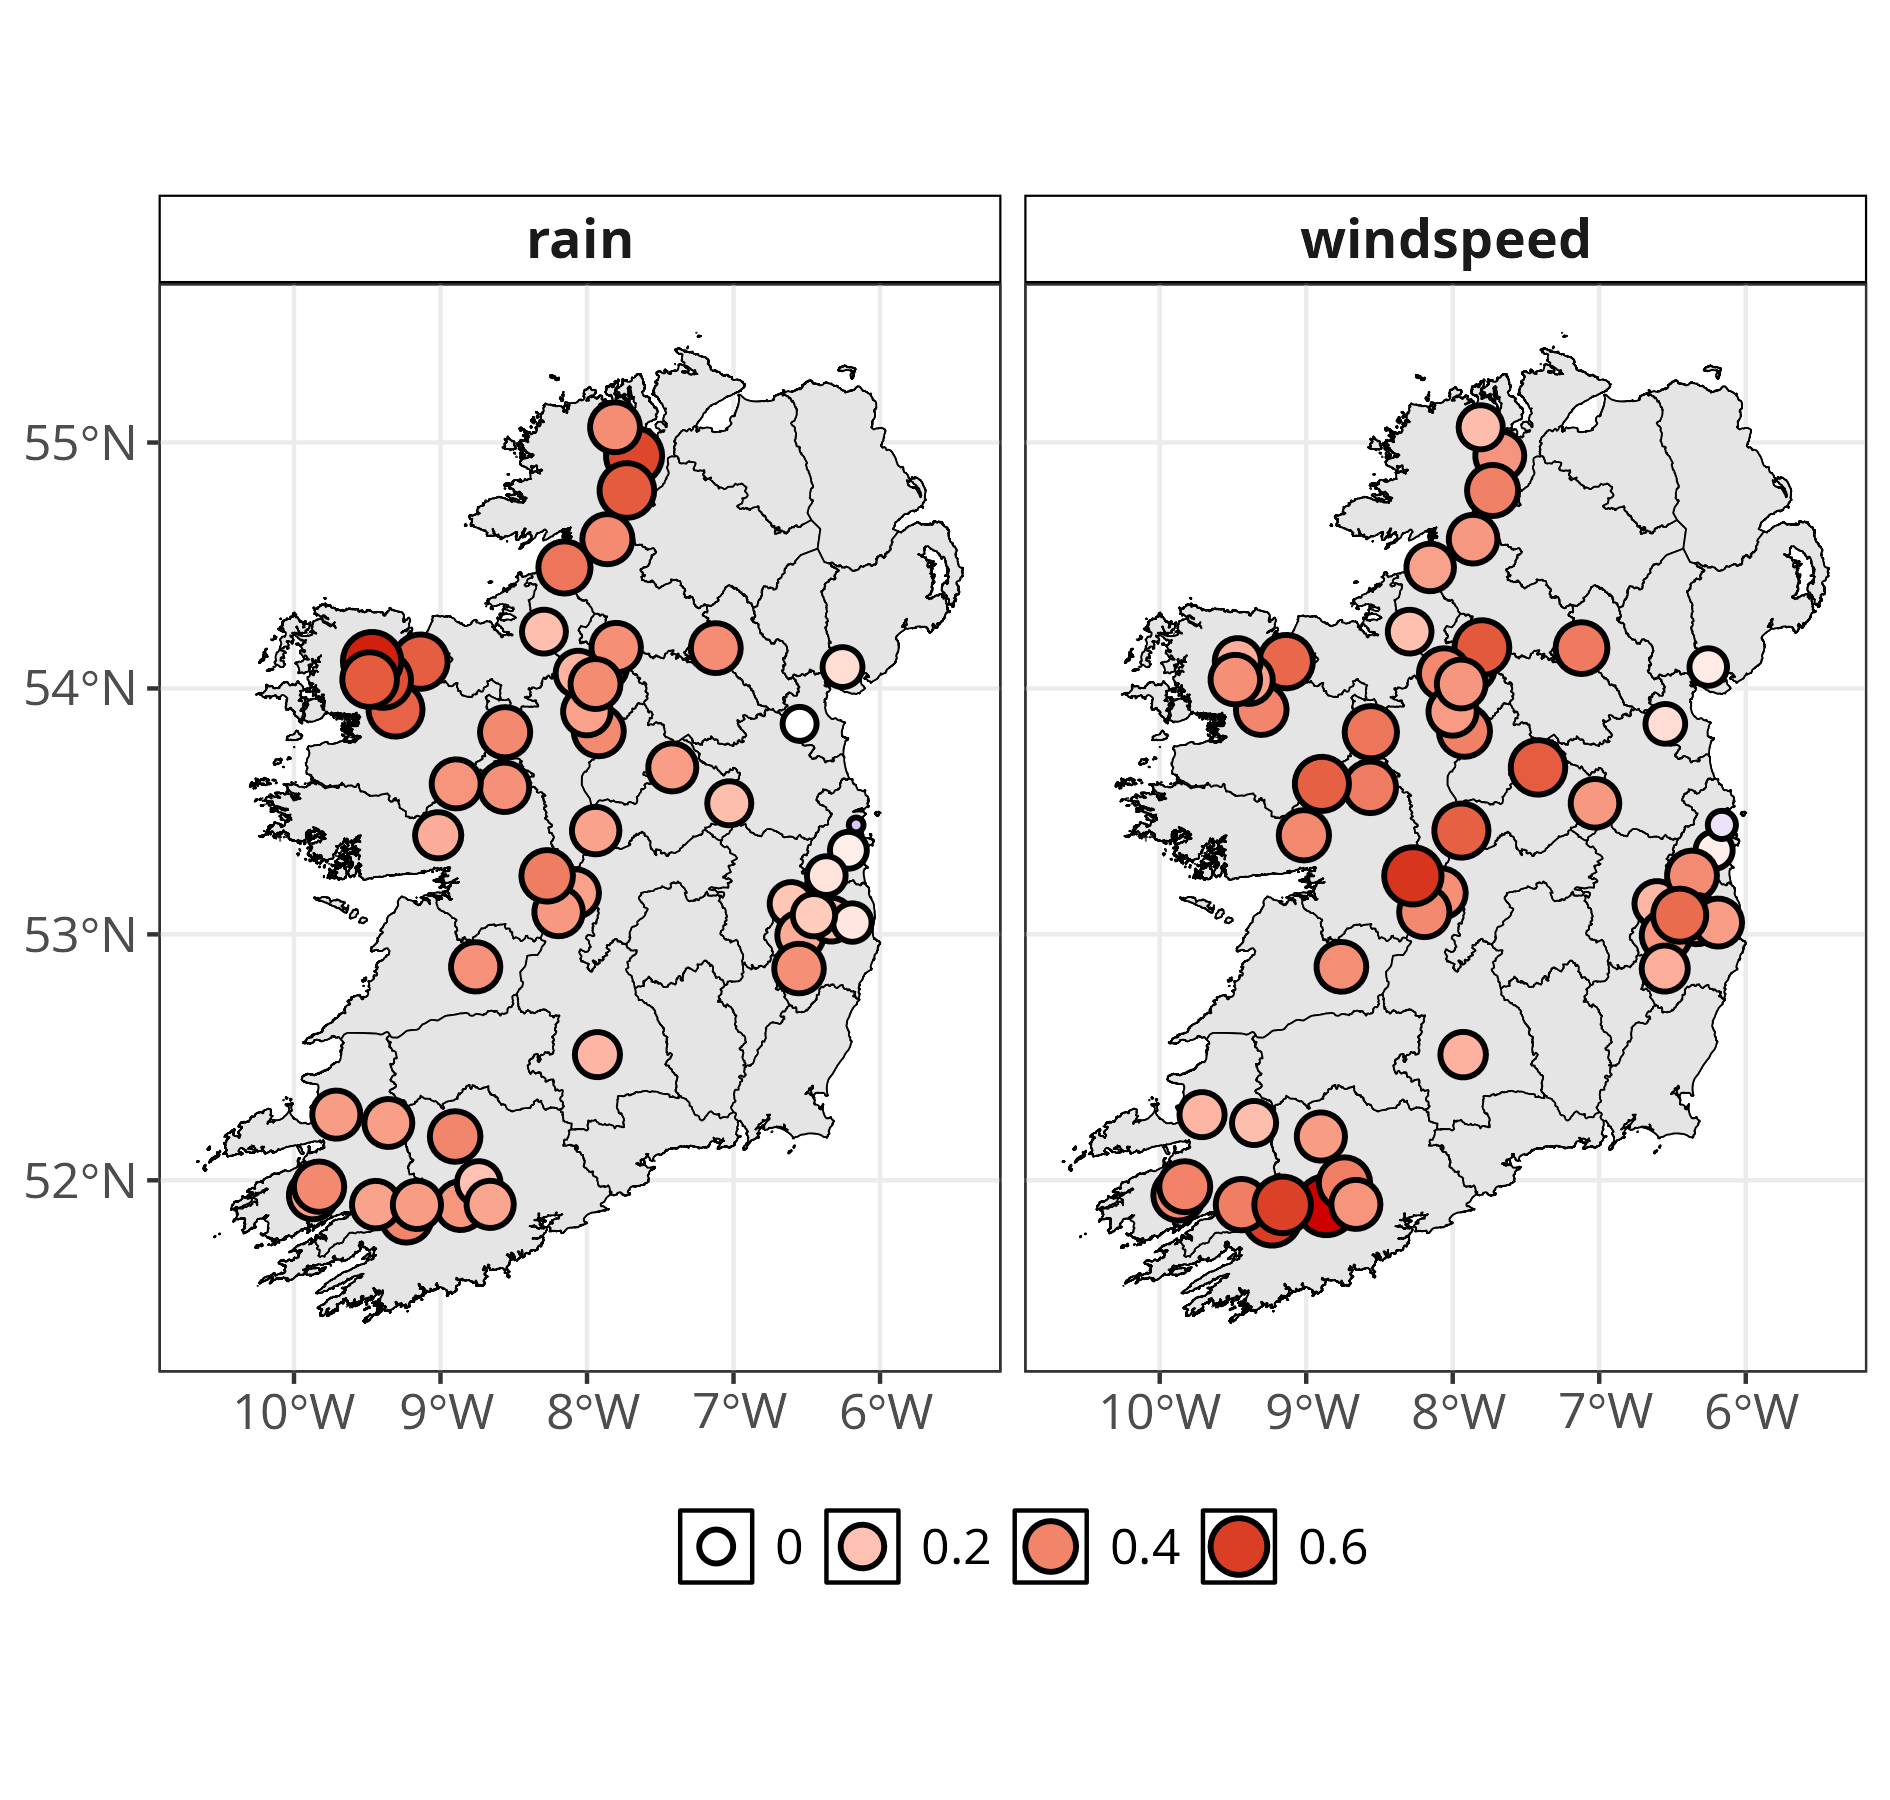
\includegraphics[width=0.99\textwidth]{plots/045_alpha_map.png}
\end{frame}

% Rain vs wind speed alpha vals, and vs lon/lat
\begin{frame}{Interpretation}
\begin{minipage}{0.49\textwidth}
        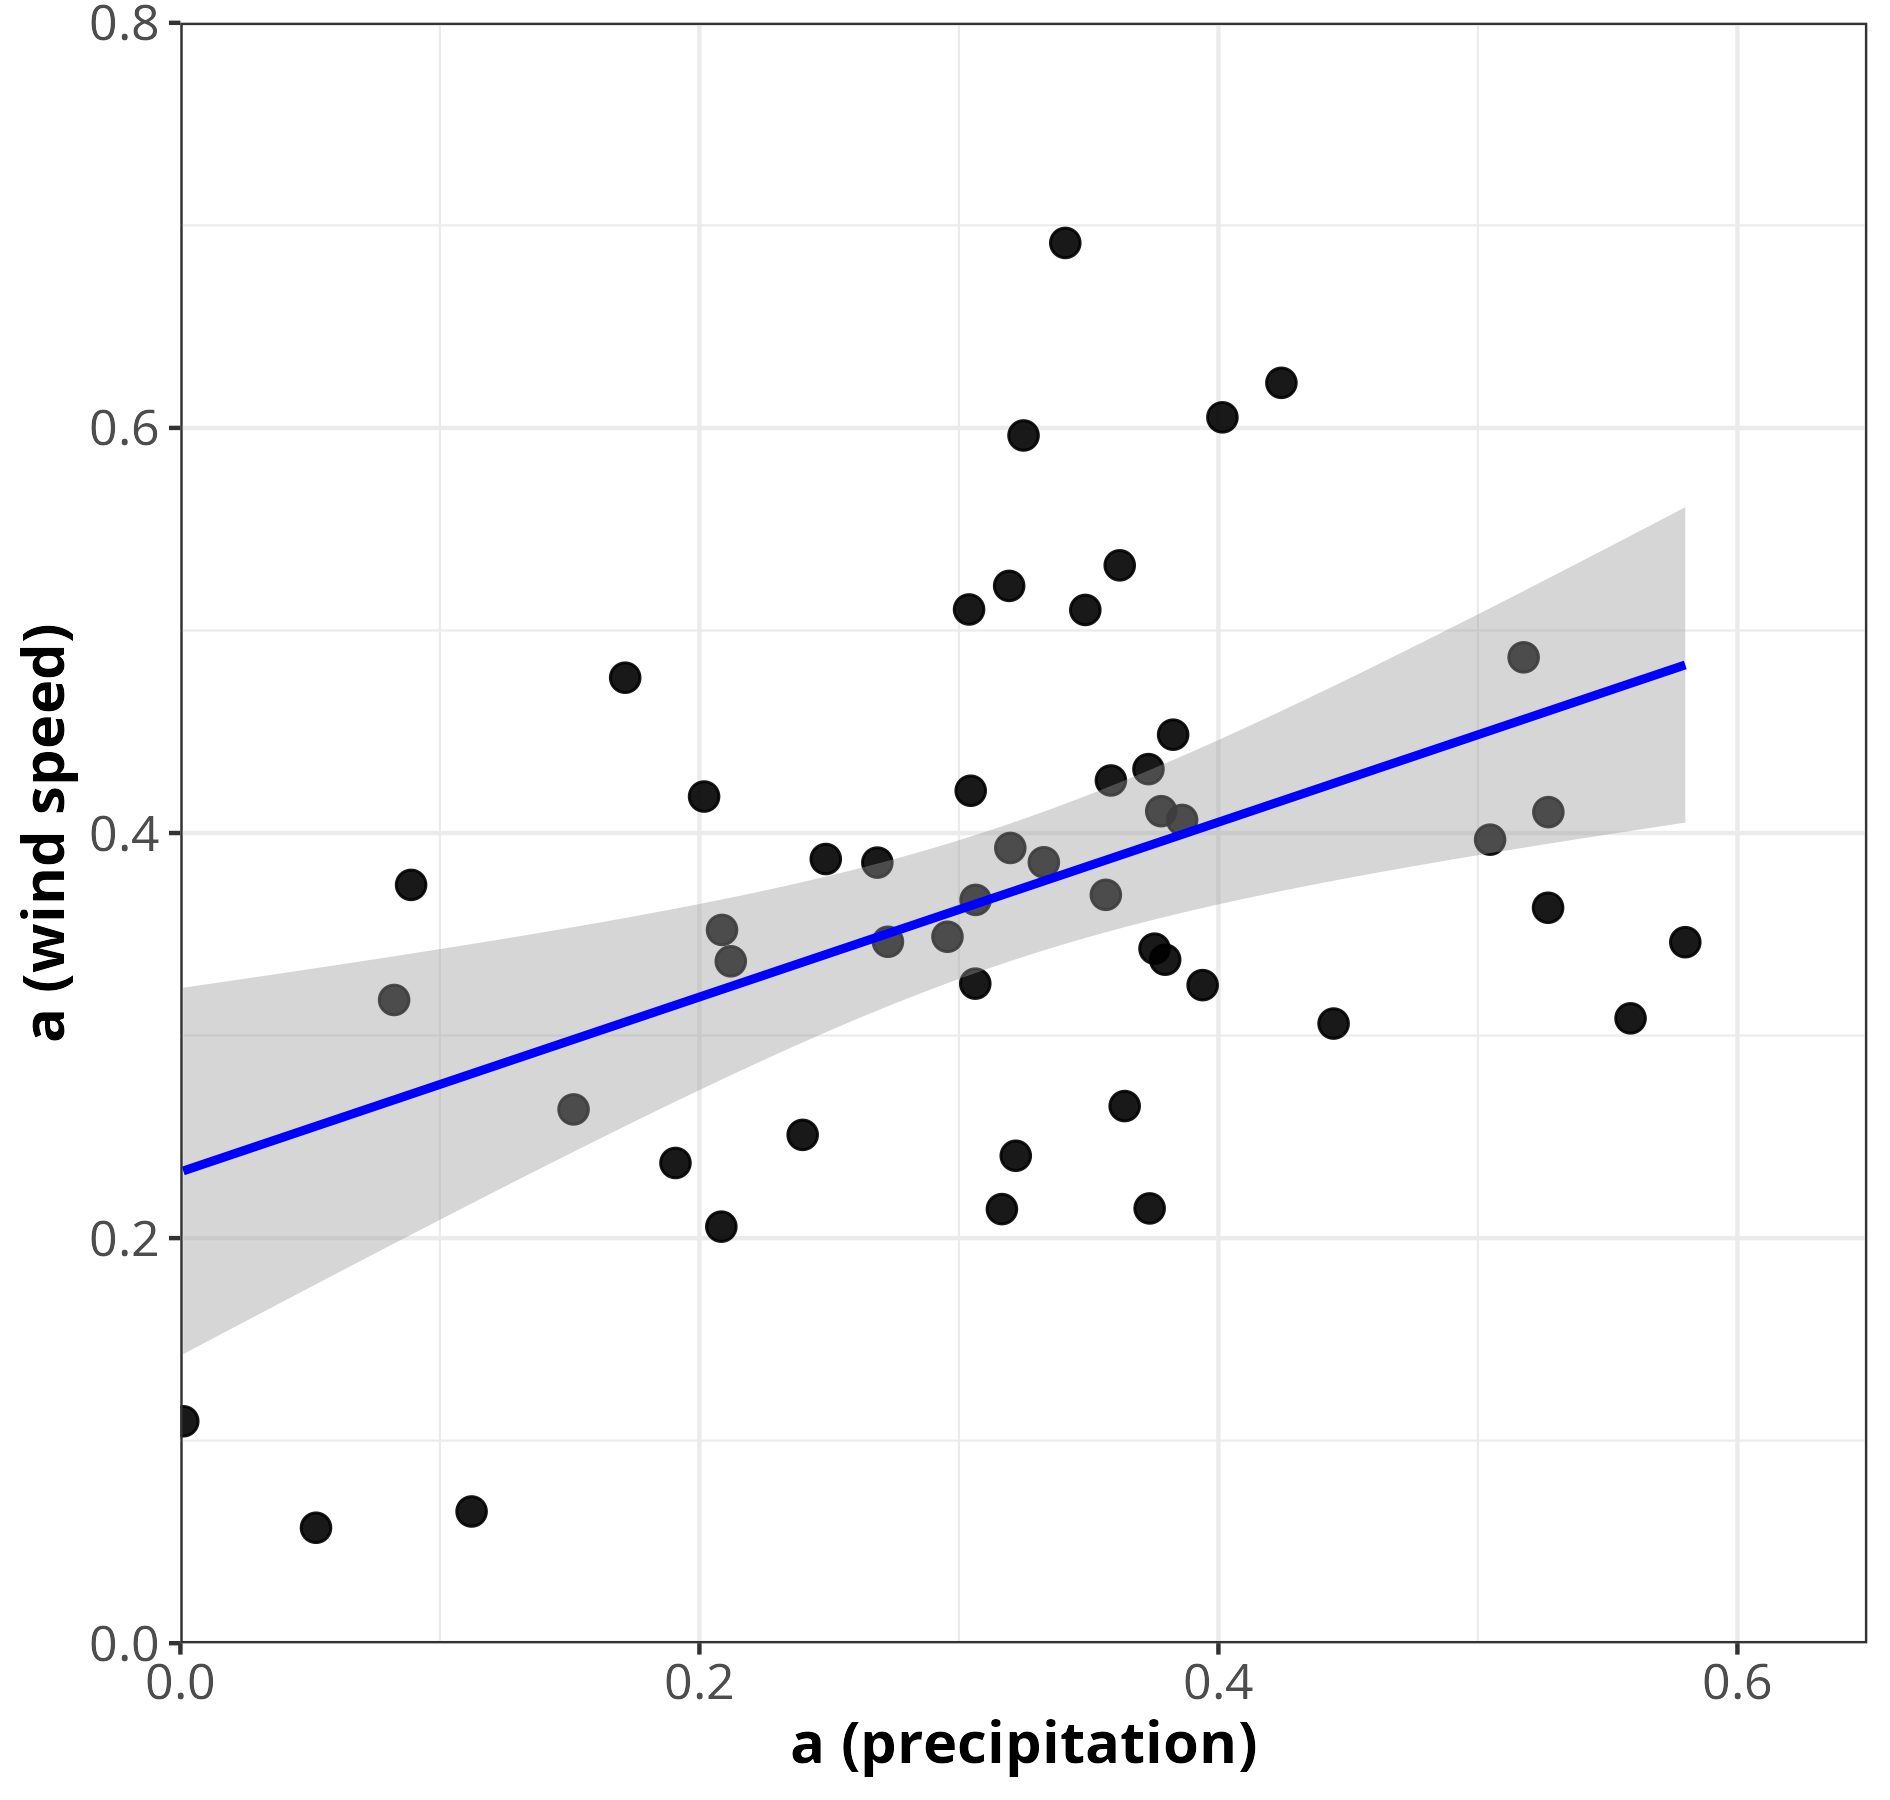
\includegraphics[width=0.99\textwidth]{plots/046_alpha_rain_vs_ws.png}
   \end{minipage}
\hfill
\begin{minipage}{0.49\textwidth}
    \begin{itemize}
        \item High values of $\alpha$ for wind speed seem to be positively correlated with high values for rainfall, indicating locations where concurrent extremal events are more common
        \item Extreme rainfall is more likely to occur along with high wind speeds the further West you travel
        % todo: Anything else?
    \end{itemize}
\end{minipage}
\end{frame}

% Briefly talk about extensions to model
% \begin{frame}{Extensions to CE model}
% \end{frame}

% TODO: May need more information/slides here
\section{Clustering}

% Reasons for and types of clustering 
\begin{frame}{Clustering}
    \begin{itemize}
        \item There are extensions to CE model which seek to overcome shortcomings of ``vanilla'' model, such as spatial and spatio-temporal versions.
        \item Alternative/additional approach: clustering
        \item Clustering done for two main reasons: to enhance the explainability and interpretation of data, and to improve parameter estimation
    \end{itemize}
\end{frame}

\begin{frame}{Explanatory clustering}
\begin{minipage}{0.49\textwidth}
    \begin{itemize}
        \item Mainly derives distance metric to perform clustering like k-means, k-mediods, and have user-defined cluster number
        \item Bernard et.\ al.\ (2013) \cite{Bernard2013} uses the F-madogram (extremal variogram) as distance measure % forms a copula
        \item Vignotto et.\ al.\ (2021) \cite{Vignotto2021} computes KL divergence for risk functions of transformed bivariate rainfall and wind speed observations for different raster locations in UK and Ireland
    \end{itemize}
\end{minipage}
\hfill
\begin{minipage}{0.49\textwidth}
    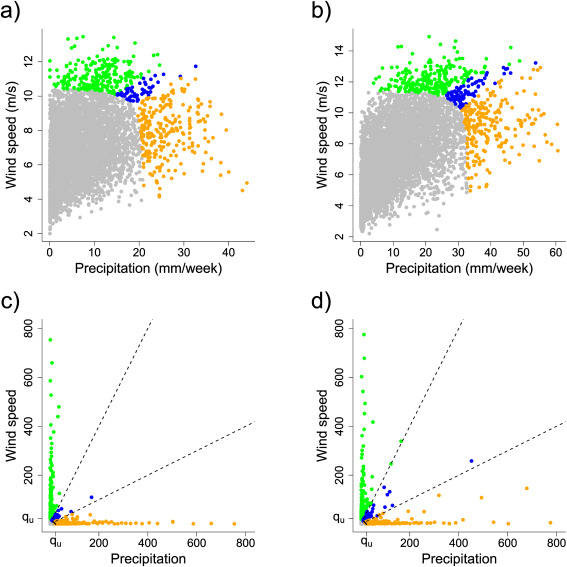
\includegraphics[width=0.99\textwidth]{images/vignotto2021.jpg}
    \caption{\emph{Source: \cite{Vignotto2021}}}
\end{minipage}
\end{frame}

\begin{frame}{Hierarchical clustering}
\begin{itemize}
    \item Seeks to find (latent, data-driven) groupings over which parameter inference is optimised
    \item In Frequestist setting, EM algorithm often used to sequentially maximise likelihood over group membership and within-group parameters (Carreau et.\ al.\ (2017) \cite{Carreau2017}, Dupuis et.\ al.\ (2023) \cite{Dupuis2023}) % conditional mixture of GPDs, GEV for panel data
    \item In Bayesian setting, one method includes using Reversible Jump MCMC algorithm which estimates number of clusters and cluster membership as latent variables (Rohrbeck, Tawn (2021) \cite{Rohrbeck2021})
    \item Need for priors can be seen as both a strength and a weakness, but the use of distributions improves uncertainty estimation % Can enforce spatial continuity
\end{itemize}
\end{frame}

\section{Conclusions and future work}

\begin{frame}{Conclusions and future work}
  \textbf{Conclusions}
    \begin{itemize}
        \item Conditional extremes model explained and shown with motivating example 
        \item ``Hacks'' required to get reasonably interpretable results with ``vanilla'' model
        \item Lit review of clustering within extremes , some promising methods found
    \end{itemize}
% \end{frame}
% 
% \begin{frame}{Future work}
    \textbf{Future Work}
    \begin{itemize}
        \item Perform k-mediods similar to \cite{Vignotto2021} on conditional extremes regression line, where KL divergence appears to be appropriate distance metric, compare results
        \item Derive Bayesian clustering algorithm similar to \cite{Rohrbeck2021}
        \begin{itemize}
            \item Sensible initial prior distribution for $Z$ is the multivariate Normal distribution, will assess suitability in practice
        \end{itemize}
        \item If successful, expand schemes to extended conditional extremes models
    \end{itemize}
\end{frame}

% TODO: Add references!
\begin{frame}\frametitle{References}
\tiny
\bibliographystyle{unsrt}
\bibliography{library.bib}
% \nocite{cocoaprod, dunn2012hadisd, faostat, hersbach2020era5, wilson2019simulation}

\end{frame}

% ===========================================================
% \frame{
% \vskip30mm
% \centerline{\Large\color{violet}\textsc{Thank you!}}
% \centerline{\Large\color{violet}\textsc{Any Questions?}}
% \vskip40mm
% }

\end{document}
